\section{Evaluation}
\label{sec:evaluation}

We depicted time relative to a window of 3 for selected values in this paper for
1MBps, 5MBps and 100MBps in figures \ref{fig:bandwith-1mb},
\ref{fig:bandwith-5mb} and \ref{fig:bandwith-100mb}. Graphs and raw data of the
whole measurement can be also lookuped on this page:
\url{https://mic92.github.io/acto15-tcpicw/}

As expected changing the initial window size for rather small and big request
sizes did not result in an improvement of request time. For small sizes
($\leq{}4\text{kiB}$) the initial window of 3 is already sufficient to transmit
all values within 1 round trip time. For bigger requests
($\gtrsim{}2048\text{kiB}$) TCP Slow Start algorithm has enough time to scale up
to the bandwidth limit.

If we look at for web more common request sizes (16kiB-256kiB), we the see
performance improves between 10\% and 20\% for a initial TCP window of 10
segments. The saving is higher, if the link latency gets higher or the link
provides more bandwidth. Therefor connections with a high Bandwith-Delay-Product
profits the most from a bigger initial congestion window. This behavior is a
consequence of equation~\ref{transfer_time}. Improving the window size beyond 10
segments still improves the user latency so it saves up 30\%-40\% of time for
window sizes like 32 and 40. However the scaling is not linear, which is also
consistent with the model~\ref{transfer_time}.

\begin{figure*}[ht]
\begin{center}
\footnotesize
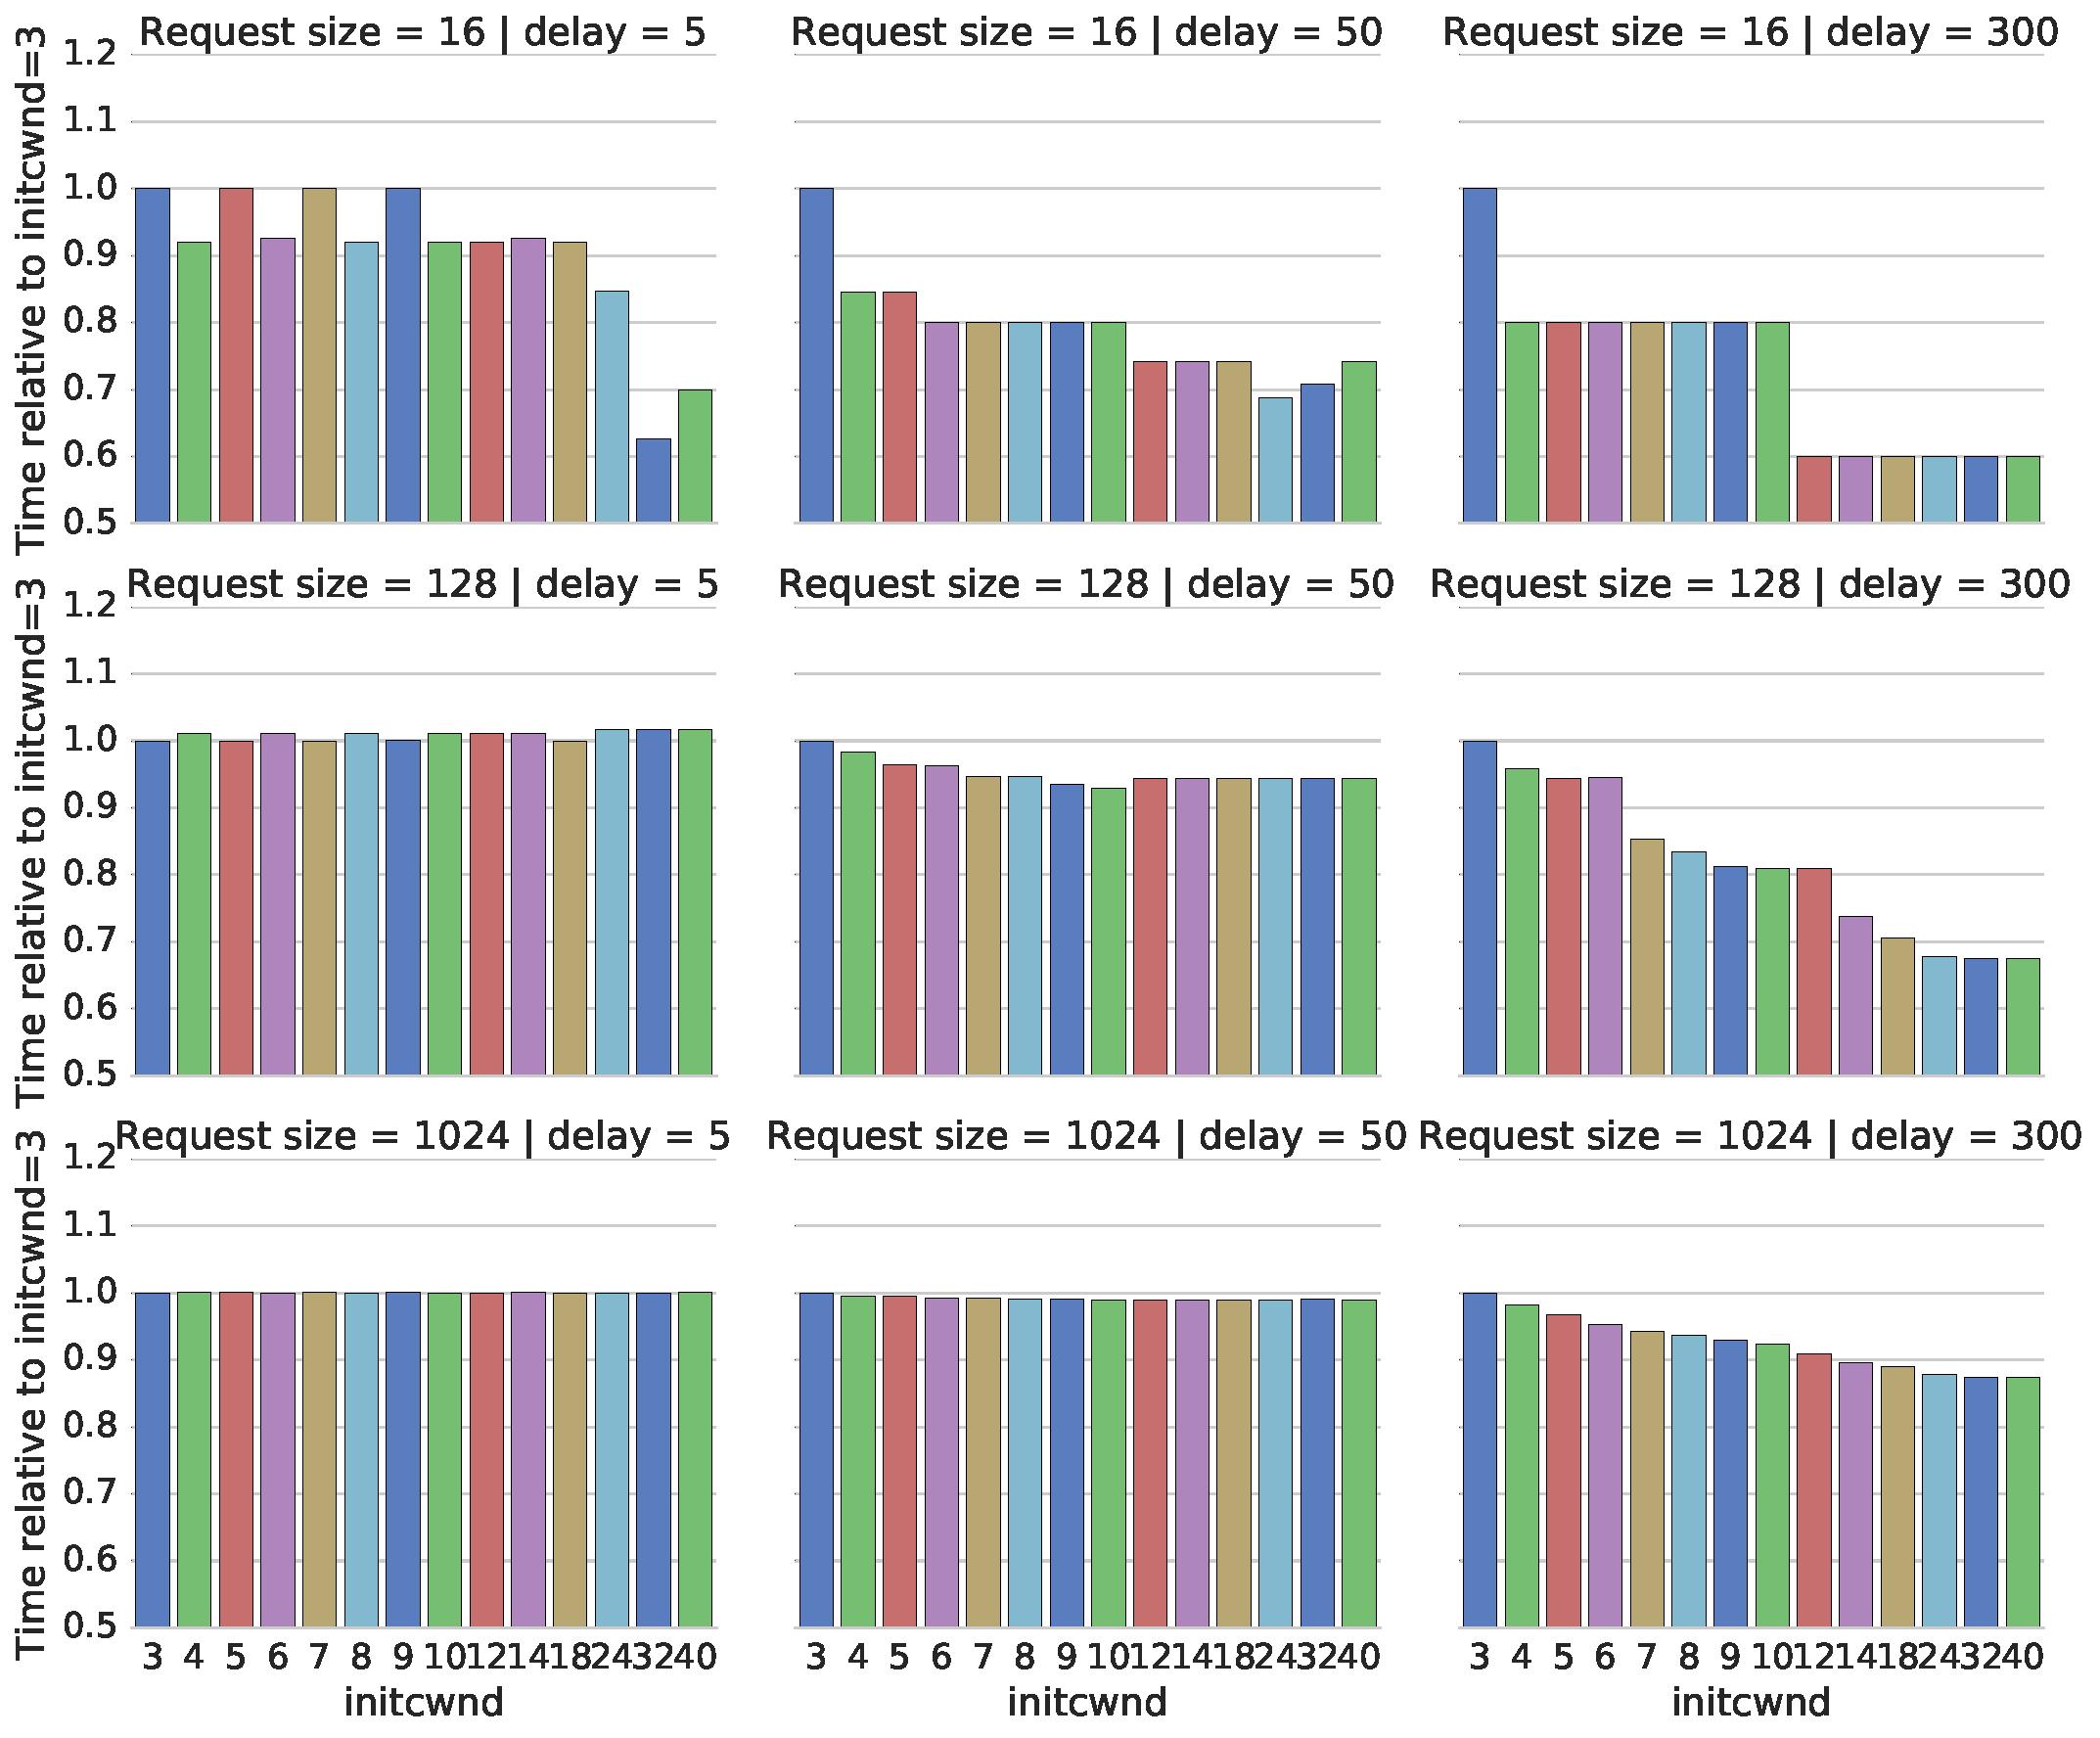
\includegraphics[scale=0.35]{figure/bandwidth-1mb}
\caption{Request time relative to a window of 3 segments with a bandwidth of
1MBps with varying forwarding delay [seconds] and varying request size [kiB]}
\label{fig:bandwith-1mb}
\end{center}
\end{figure*}

\begin{figure*}[ht]
\begin{center}
\footnotesize
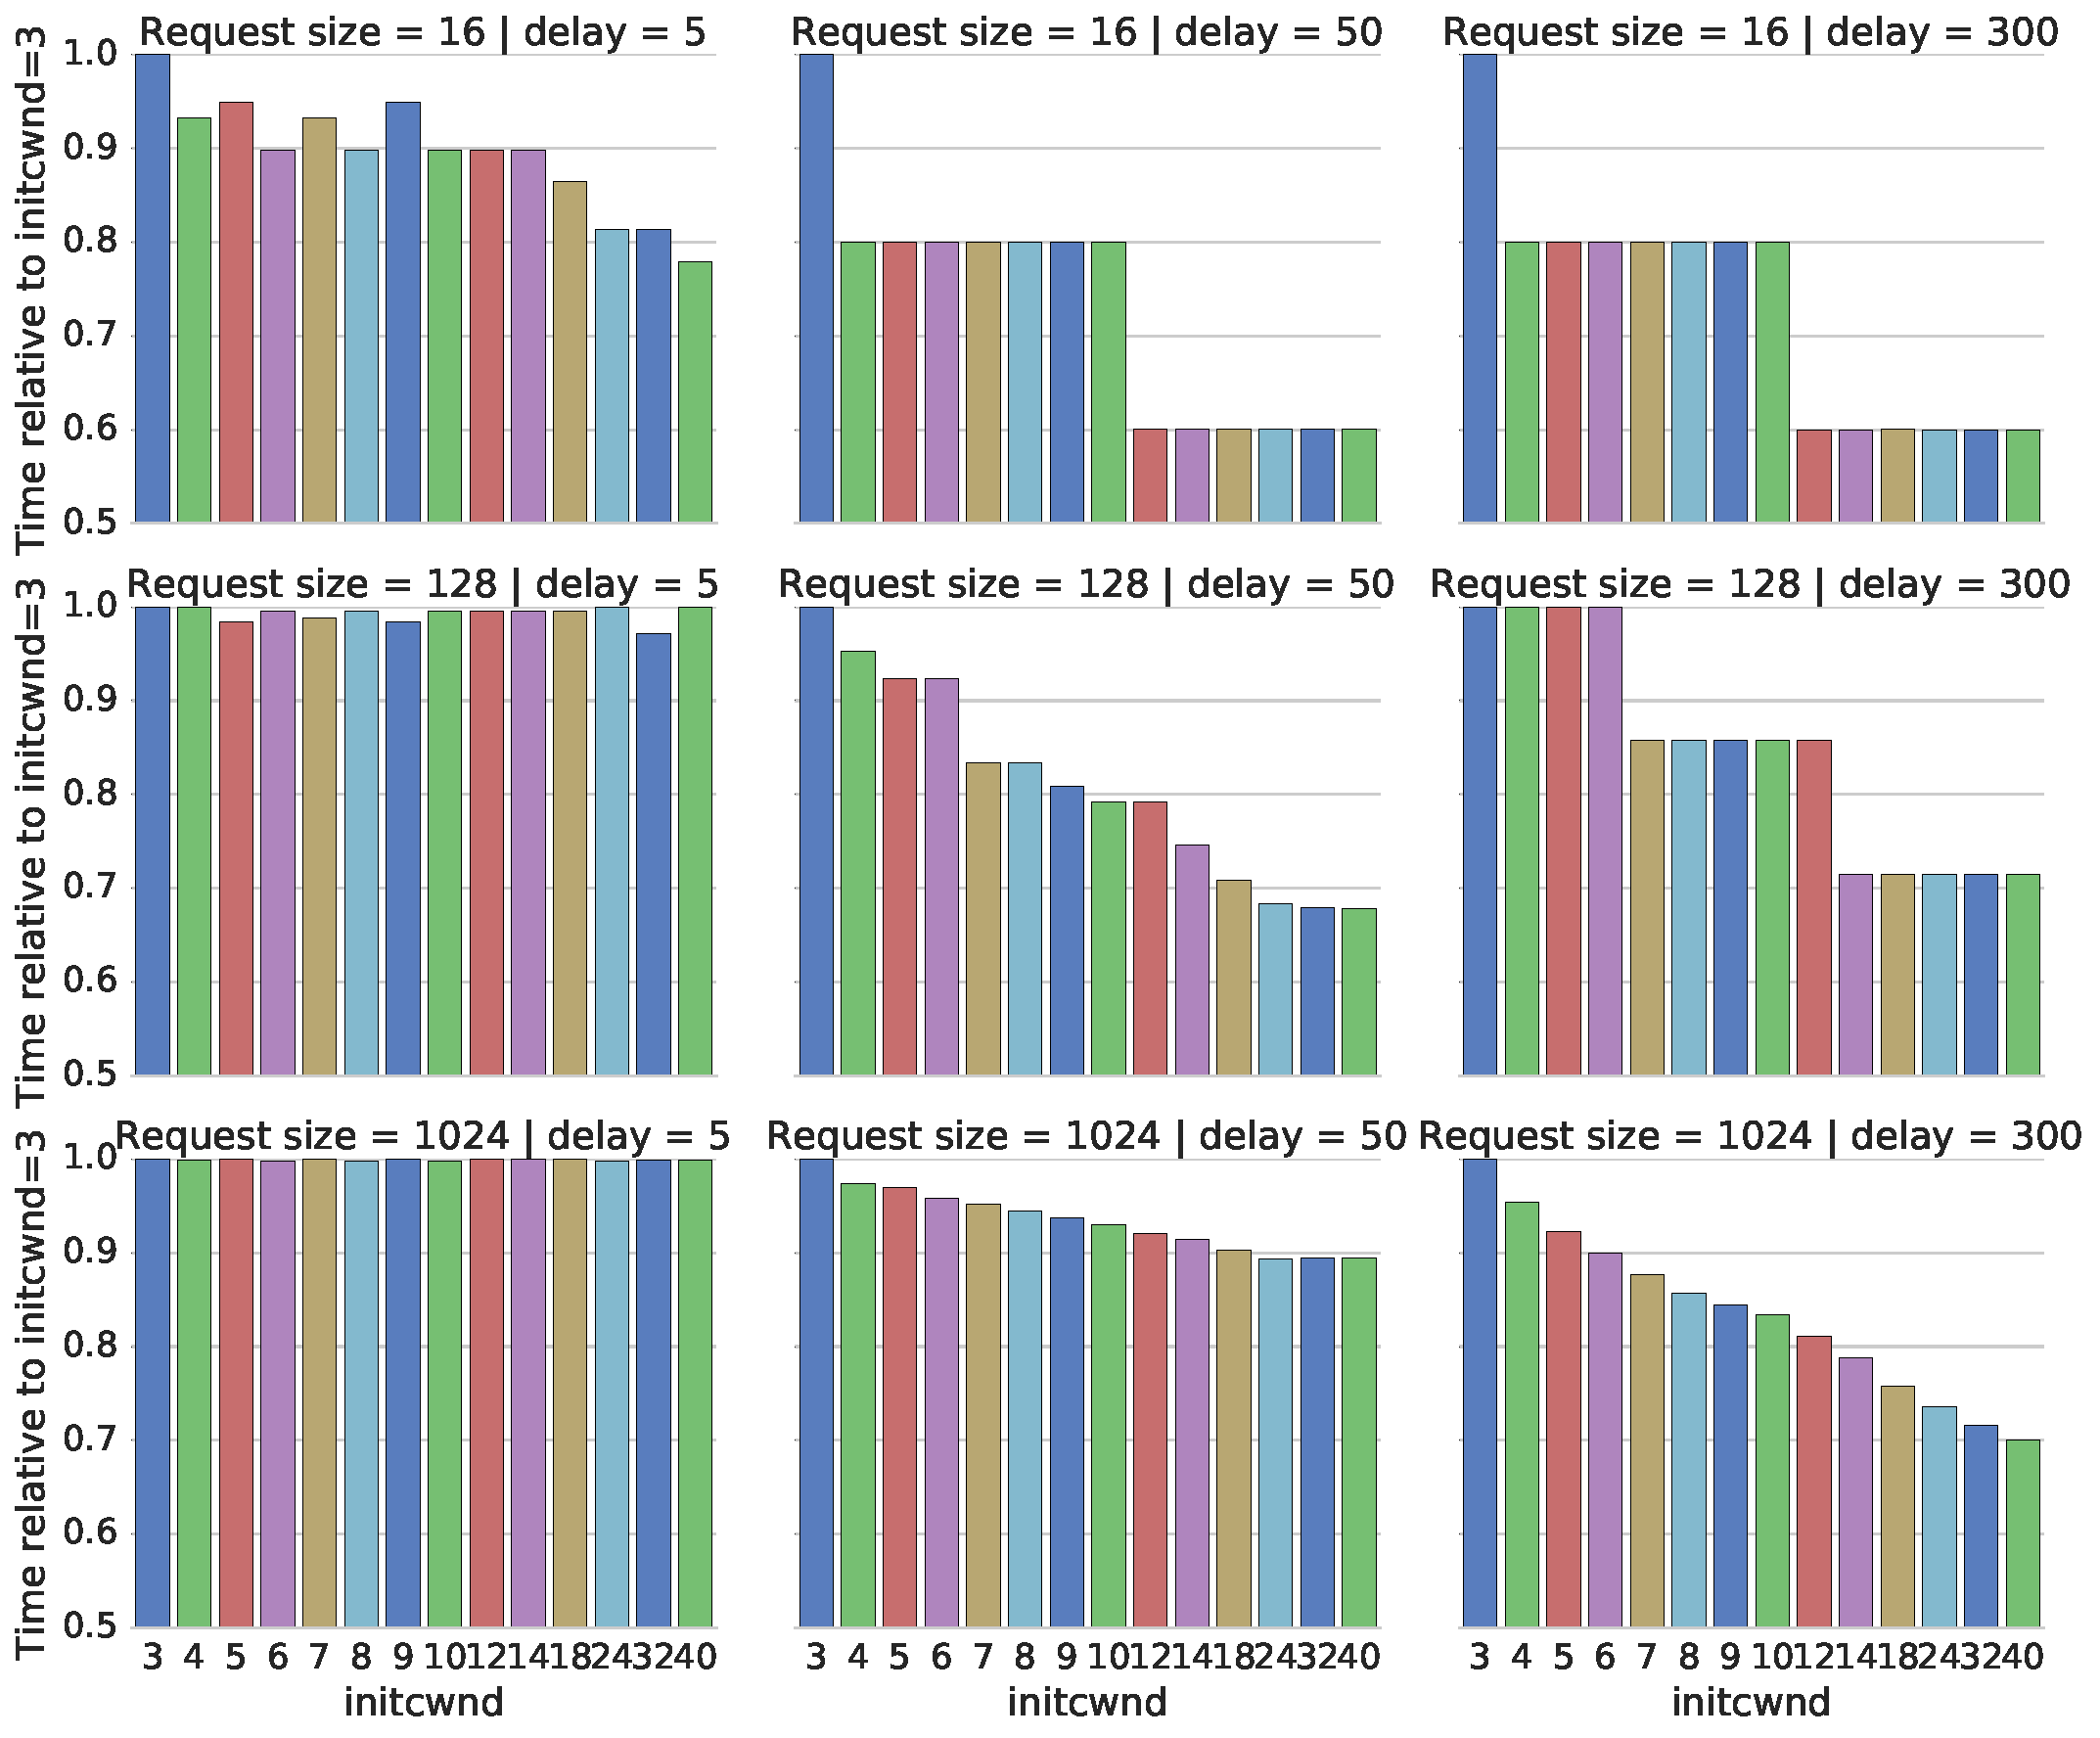
\includegraphics[scale=0.35]{figure/bandwidth-5mb}
\caption{Request time relative to a window of 3 segments with a bandwidth of
5MBps with varying forwarding delay [seconds] and varying request size [kiB]}
\label{fig:bandwith-5mb}
\end{center}
\end{figure*}

\begin{figure*}[ht]
\begin{center}
\footnotesize
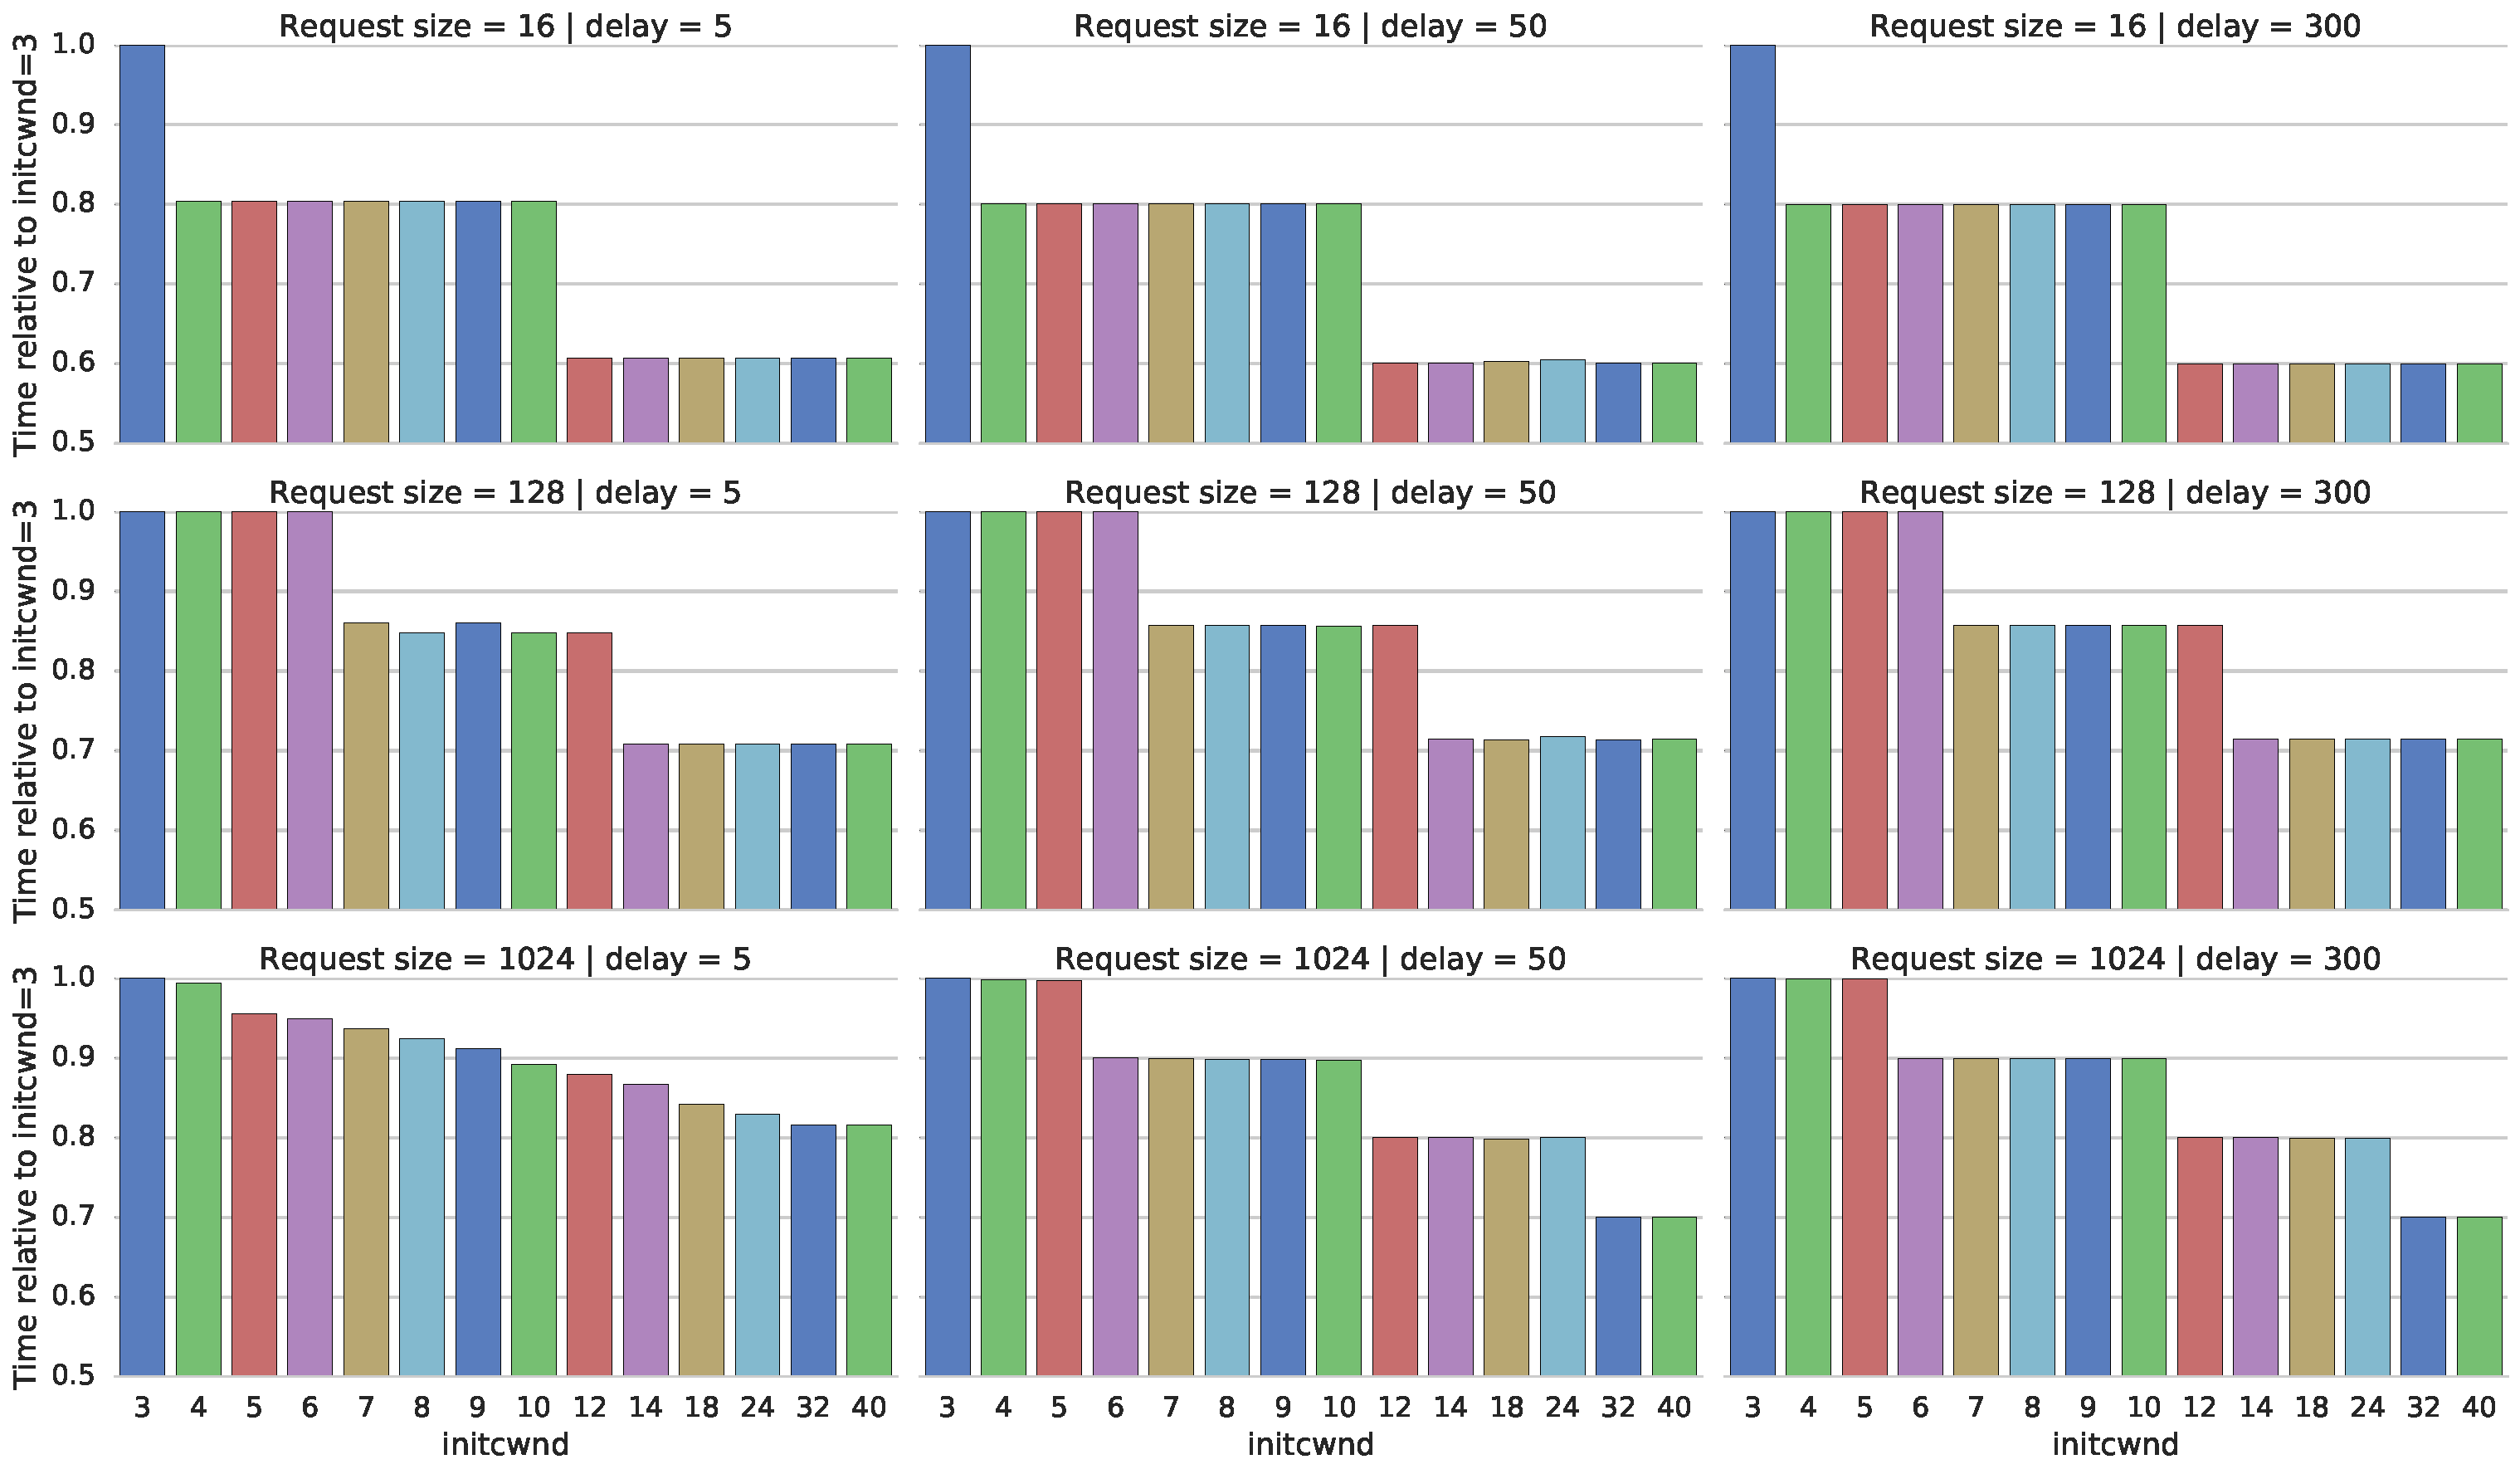
\includegraphics[scale=0.35]{figure/bandwidth-100mb}
\caption{Request time relative to a window of 3 segments with a bandwidth of
100MBps with varying forwarding delay [seconds] and varying request size [kiB]}
\label{fig:bandwith-100mb}
\end{center}
\end{figure*}


%# Testsetup
%
%## Grenzen der Simulation:
%- Nur ein Link zum Server simuliert
%  -> aber häufig der Flaschhals zwischen Client und Server
%- Nur den Linux-TCP Stack und dessen Standardeinstellungen betrachtet
%- Nur symmetrische Bandbreiten getestet
%  -> sollte keinen Einfluss haben,
%  da Acknowledges verhältnissmäßig zur übertragenen Nachricht klein sind.
%
%- bw = (cwnd * mtu) / rtt
